\section{Bipolar transistors}
A byproduct of the Bulk CMOS structure is a pair of parasitic bipolar transistors.\footnote{\url{http://www.analog.com/en/analog-dialogue/articles/winning-the-battle-against-latchup.html}}
The collector of each BJT is connected to the base of the other transistor in a positive feedback structure.
A phenomenon called latchup can occur when both BJT's conduct, creating a low resistance path between VDD and GND and the product of the gains of the two transistors in the feedback loop $\beta_1 \times \beta_2$ is greater than one.
The result of latchup is at the minimum a circuit malfunction, and in the worst case, the destruction of the device.

\begin{figure}[H]
	\centering
	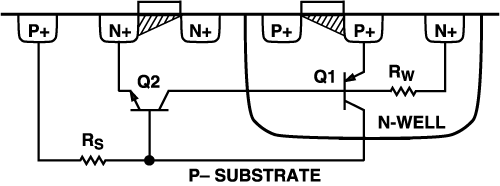
\includegraphics[scale=0.5]{latchup_cross.png}
	\caption{Lateral and vertical parasitic BJT}
	\label{latchup_diagram}
\end{figure}

In \autoref{latchup_diagram} we can see the two above mentioned transistors. In order to find out their average $\beta$ we split it up into two separate test circuits, allowing us to measure their properties out with probes on our test wafer.

\subsection{Lateral bipolar transistor}

We split out the lateral bipolar junction transistor for testing.

\begin{figure}[H]
	\centering
	\begin{tikzpicture}[node distance = 3cm, auto, thick,scale=0.5, every node/.style={transform shape}]
		% substrate
\fill[substrate] (0,0) rectangle (11,2);
\node at (2,0.5) {Silicon substrate};
%trenches
\fill[isolationoxide] (0,0.75) rectangle (1.25,2);
\fill[isolationoxide] (3.75,0.75) rectangle (5,2);
\fill[isolationoxide] (10.5,0.75) rectangle (11,2);
% n-well
\fill[nwell] (1.25,0.75) rectangle (3.75,2);
\node at (2,1) {N-Well};
\fill[nimplant] (1.5,1.5) rectangle (3.5,2);
\node at (2,1.65) {n+};
% p-well
\fill[pwell] (5,0.75) rectangle (10.5,2);
\node at (6,1) {P-Well};

\fill[nimplant] (5.25,1.5) rectangle (7.25,2);
\node at (6,1.65) {n+};

\fill[pimplant] (8.25,1.5) rectangle (10.25,2);
\node at (9,1.65) {p+};

\draw (6.25,1.5) -- (6.25,0) to[Tnpn,n=npn] (2.5,0) -- (2.5,1.5);

\draw (npn.B) -- +(5,0) -- (9.25,1.5);
	\end{tikzpicture}
	\caption{Lateral BJT cross section}
	\label{lateral_bjt_cross_section}
\end{figure}

In \autoref{lateral_bjt_cross_section} the cross section of our testing circuit can be seen.
Now we can characterize the $\beta$ value of the lateral bipolar transistor all over the wafer and get a good approximation of the worst case conditions.

\subsection{Vertical bipolar transistor}

We split out the vertical bipolar junction transistor for testing.

\begin{figure}[H]
	\centering
	\begin{tikzpicture}[node distance = 3cm, auto, thick,scale=0.5, every node/.style={transform shape}]
		% substrate
\fill[substrate] (0,0) rectangle (11,2);
\node at (2,0.5) {Silicon substrate};
%trenches
\fill[isolationoxide] (0,0.75) rectangle (1.25,2);
\fill[isolationoxide] (5.75,0.75) rectangle (7,2);
\fill[isolationoxide] (9.5,0.75) rectangle (11,2);
% n-well
\fill[nwell] (1.25,0.75) rectangle (5.75,2);
\node at (2,1) {N-Well};

\fill[nimplant] (1.5,1.5) rectangle (3.5,2);
\node at (2,1.65) {n+};
\fill[pimplant] (3.5,1.5) rectangle (5.5,2);
\node at (5,1.65) {p+};

% p-well
\fill[pwell] (7,0.75) rectangle (9.5,2);
\node at (9,1) {P-Well};
\fill[pimplant] (7.25,1.5) rectangle (9.25,2);
\node at (9,1.65) {p+};

\draw  (8.25,1.5) -- (8.25,-1.5) -- (4.5,-1.5) to[Tpnp,n=pnp] (4.5,1.5);

\draw (pnp.B) -- +(-1.15,0) -- (2.5,1.5);
	\end{tikzpicture}
	\caption{Vertical BJT cross section}
	\label{vertical_bjt_cross_section}
\end{figure}

In \autoref{vertical_bjt_cross_section} the cross section of our testing circuit can be seen.
Now we can characterize the $\beta$ value of the vertical bipolar transistor all over the wafer and get a good approximation of the worst case conditions.
